\documentclass[]{beamer}
%language
\usepackage[ngerman,english]{babel}
\usepackage[utf8]{inputenc}

%\usepackage[usenames,dvipsnames]{xcolor}

\usepackage{tikz}
\usetikzlibrary{shapes}
\usetikzlibrary{mindmap}

\usepackage[utf8]{inputenc}
%theme
\useoutertheme[nofootline]{wuerzburg}
\useinnertheme{chamfered}
\usecolortheme{shark}

%title setup
\title{Generischer Titel: Studie - Emailkryptographie}
%\subtitle{Montag 12-14, Raum 01.150-128}
\subtitle{Human Factors in IT-Security}
\author{Ulrich Dorsch, Tim Grocki, Leonhard Hösch  \\ {\tiny ulrichdorsch@googlemail.com, tgrocki@lavabit.com, lh@dancingwolf.de \\}}
\institute[Universität Erlangen]{Friedrich-Alexander-Universität Erlangen
\\Department Informatik \\ Lehrstuhl 1}


\AtBeginSection[]
{
	\begin{frame}
		\frametitle{Inhalt}
		\tiny{\tableofcontents[currentsection]}
	\end{frame}
}

\definecolor{goldenrod}{HTML}{FFDF42}

\begin{document}

\begin{frame}[plain]
	\begin{center}
		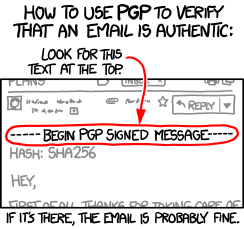
\includegraphics[scale=0.7]{pic/pgp.png}\phantom{\footnote{\url{http://xkcd.com/1181/}}}
	\end{center}
\end{frame}

%titlepage
\begin{frame}[plain]
	\titlepage
\end{frame}


\section{Zielsetzungen der Studie}

\subsection{Motivation}
\begin{frame}{Motivation}
\begin{itemize}
	\item E-Mail-Kryptographie ist nicht weit verbreitet, obwohl es viele Gründe für deren Einsatz gibt.
	\item Es wird oft vermutet, dass schlechte Benutzerfreundlichkeit der Grund für die geringe Verbreitung ist.
	\item Wir haben dies mit unserer Studie überprüft.
\end{itemize}
\end{frame}


\subsection{Forschungsfrage}
\begin{frame}{Forschungsfrage}
	Sind Usability-Probleme tatsächlich die Hauptgründe für die geringe Verbreitung von E-Mail-Kryptographie?

	\vspace{1.2cm}
	\onslide<2>{Welche anderen Ursachen spielen eine (wie große) Rolle?}
\end{frame}

\subsection{Hypothese}
\begin{frame}{Hypothese}
	Usability-Probleme im Zusammenhang mit Kryptographie-Software sind
   nicht die primäre Ursache für die geringe Verbreitung von E-Mail-Kryptographie,
   da mehr als 50\% der potenziellen Nutzer durch andere Ursachen davon abgehalten werden, E-Mail-Kryptographie zu nutzen.
	\onslide<2>{
		\begin{block}{Usability-Problem -- Definition}
			In unserem Kontext betrachten wir ein Usability-Problem als eine technische Hürde,
			die die Benutzung von E-Mail-Kryptographie verhindert oder deutlich erschwert.
		\end{block}
	}
\end{frame}

\section{Umfrageumstände}
%% NSA
\begin{frame}{NSA-Skandal}
	\begin{itemize}
	\item Der NSA-Skandal ging im Zeitraum unserer Umfrage durch alle Medien
		\footnote{\url{http://www.tagesschau.de/ausland/spionageaffaere100.html}}
	\item Überwachung des Internets, insbesondere von E-Mails
	\item Überwachung auch in Deutschland
	\item $\Rightarrow$ Erhöhtes Bewusstsein für IT-Sicherheit und die Existenz von
		Eingriffen in die Privatsphäre
	\end{itemize}
\end{frame}

\section{Demographische Daten}
\begin{frame}{Zielgruppe}
	Studierende (an der technischen Fakultät der Universität Erlangen)
\onslide<2>{
	\begin{itemize}
		\item einfach zu erreichen
		\item höchstwahrscheinlich aktive Nutzer von E-Mailkommunikation
		\item ``zukünftige Elite Deutschlands''
		\item ca. 9000 Personen
	\end{itemize}
}
\end{frame}

\begin{frame}{Rücklauf}
	\begin{itemize}
		\item 207 vollständige und verwertbare Rückläufer
		\item ca. $2,3\%$ der vorhandenen Zielgruppe
		\item Rückläufer aus diversen Studienfächern
	\end{itemize}
\end{frame}

\begin{frame}{Demographische Daten}
	\begin{center}
		Studienfächer
	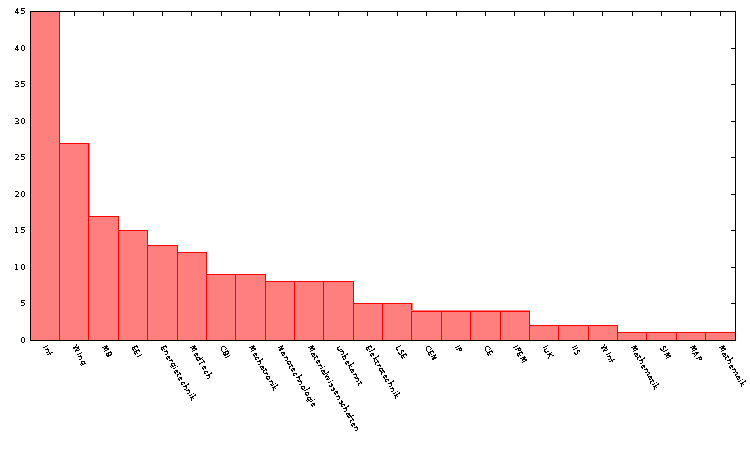
\includegraphics[scale=0.9]{plots/stud.pdf}
	\end{center}
\end{frame}

\section{Auswertung der Antworten}
\subsection{Interesse an E-Mail-Kryptographie}
\begin{frame}{Interesse an E-Mail-Kryptographie}
	\begin{center}
		\only<1>{Halten Sie das Verschlüsseln von E-Mails für sich persönlich für sinnvoll?\\
			\vspace{1cm}
				Ja: 51\% Nein: 41\% N/A: 08\%
		}
		\only<2>{Halten Sie das Verschlüsseln von E-Mail im Allgemeinen für sinnvoll?\\
			\vspace{1cm}
				Ja: 87\% Nein: 06\% N/A: 07\%
		}
		\only<3>{Hätten Sie gerne die Möglichkeit, mit Banken oder ähnlichen Institutionen/Unternehmen verschlüsselt zu kommunizieren?\\
			\vspace{1cm}
				Ja: 83\% Nein: 07\% N/A: 11\%
		}
		\only<4>{Würden Sie sich wünschen, dass Unternehmen wie z.B.\ Banken intern verschlüsselt kommunizieren?\\
			\vspace{1cm}
				Ja: 85\% Nein: 06\% N/A: 09\%
		}
	\end{center}
\end{frame}

\subsection{Bekanntheit von Gefahren}
\begin{frame}{Bekanntheit von Gefahren}
	  \begin{center}
		  \only<1>{ Eine unverschlüsselte E-Mail, die Sie versenden, kann auf dem Zustellweg von einem Angreifer mitgelesen und verändert werden. \\ Wussten Sie das?\\
			  \vspace{1cm}
      Ja: 82\% Nein: 15\% N/A: 02\%
  }
  \only<2>{ E-Mails können mit sehr geringem Aufwand unter falschem Absender versendet werden, wenn diese nicht kryptographisch signiert sind. \\ Wussten Sie das?\\
	  \vspace{1cm}
      Ja: 68\% Nein: 29\% N/A: 03\%
  }
  \only<3>{ Sollte ein Angreifer (Hacker) administrative Zugriffsrechte auf den Server einer Firma erlangen kann dieser alle unverschlüsselten E-Mails der Firma lesen oder sogar verändern. \\ Wussten Sie das?\\
	  \vspace{1cm}
      Ja: 84\% Nein: 14\% N/A: 03\%
  }
  \end{center}	
\end{frame}


%%%% 'E-Mail-Kryptographie' unbekannt
\subsection{Schema des Fragebogens}

\begin{frame}[fragile]{Fragebogenverlauf}
	Der Rest des Fragebogens ist baumartig strukturiert, sodass eine Einteilung
	in verschiedene Kategorien (diverse Ursachen für geringe Verbreitung von
	E-Mail-Kryptographie) leichtfällt.

	\tikz[baseline=-0.5ex] \fill[goldenrod] (0,0) circle (2ex); Ast, der gerade betrachtet wird

	\tikz[baseline=-0.5ex] \fill[red] (0,0) circle (2ex); Blatt mit Usability-Problem

	\tikz[baseline=-0.5ex] \fill[blue!70] (0,0) circle (2ex); Blatt ohne Usability-Problem

\end{frame}

\begin{frame}{Fragebogenverlauf}
	\begin{tikzpicture}[mindmap,scale=0.7]
		\path[concept color=goldenrod,every concept/.append style={scale=0.7}]
		node[concept] (R) {$207$ \\ $100\%$}
			child[concept color=blue!70,grow=-5] {node[concept] {$65$ \\ $31.40\%$}}
			child[concept color=gray,grow=-170] {node[concept] {}
				child[concept color=gray,grow=-30] {node[concept] {}
					child[concept color=gray,grow=-90] {node[concept] {}
						child[concept color=gray,grow=-130] {node[concept] {}}
						child[concept color=gray,grow=-70] {node[concept] {}}
					}
					child[concept color=gray,grow=-10] {node[concept] {}
						child[concept color=gray,grow=0] {node[concept] {}}
						child[concept color=gray,grow=-60] {node[concept] {}
							child[concept color=gray,grow=-130] {node[concept] {}}
							child[concept color=gray,grow=-50] {node[concept] {}}
						}
					}
				}
				child[concept color=gray,grow=-130] {node[concept] {}
					child[concept color=gray,grow=-130] {node[concept] {}}
					child[concept color=gray,grow=-70] {node[concept] {}
						child[concept color=gray,grow=-130] {node[concept] {}}
						child[concept color=gray,grow=-70] {node[concept] {}
							child[concept color=gray,grow=-130] {node[concept] {}}
							child[concept color=gray,grow=-70] {node[concept] {}}
						}
					}
				}
			};
			\only<1>{
				\draw node[annotation,below,fill=gray!30] (Q) at (-6,2.3) {Wissen Sie, was E-Mail-Kryptographie ist?};
				\draw [concept connection] (R) edge (Q);
			}
			\only<2>{
				\node[annotation,below,fill=gray!50,scale=1.3] at (4,-6.4) {Der Begriff ``E-Mail-Kryptographie'' ist unbekannt.};
			}
	\end{tikzpicture}
\end{frame}

\begin{frame}{Details}
	\begin{center}
		Studienfächer
	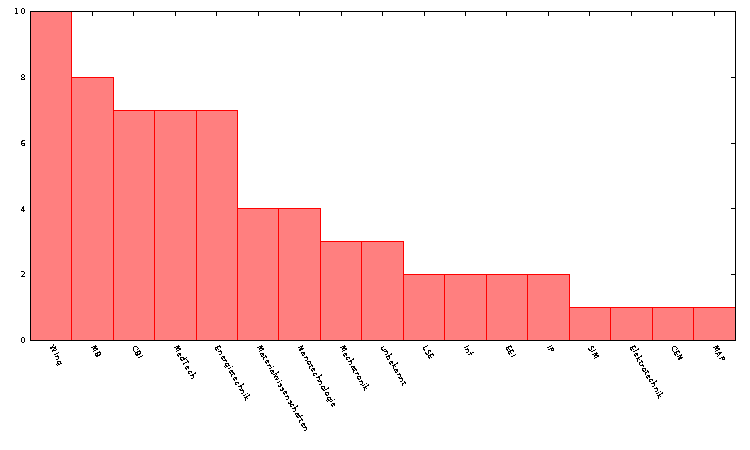
\includegraphics[scale=0.9]{plots/emailkryptunbek.pdf}
\end{center}
\end{frame}

%%%% E-Mail-Kryptographie regelmäßig eingesetzt
\begin{frame}{Fragebogenverlauf}
	\begin{tikzpicture}[mindmap,scale=0.7]
		\path[concept color=goldenrod,every concept/.append style={scale=0.7}]
		node[concept] {$207$ \\ $100\%$}
			child[concept color=gray,grow=-5] {node[concept] {$65$ \\ $31.40\%$}}
			child[concept color=goldenrod,grow=-170] {node[concept] (R) {$142$ \\ $68,60\%$}
				child[concept color=gray,grow=-30] {node[concept] {}
					child[concept color=gray,grow=-90] {node[concept] {}
						child[concept color=gray,grow=-130] {node[concept] {}}
						child[concept color=gray,grow=-70] {node[concept] {}}
					}
					child[concept color=gray,grow=-10] {node[concept] {}
						child[concept color=gray,grow=0] {node[concept] {}}
						child[concept color=gray,grow=-60] {node[concept] {}
							child[concept color=gray,grow=-130] {node[concept] {}}
							child[concept color=gray,grow=-50] {node[concept] {}}
						}
					}
				}
				child[concept color=goldenrod,grow=-130] {node[concept] (R1) {$54$ \\ $26.09\%$}
					child[concept color=blue!70,grow=-130] {node[concept] {$30$ \\ $14.49\%$}}
					child[concept color=gray,grow=-70] {node[concept] {}
						child[concept color=gray,grow=-130] {node[concept] {}}
						child[concept color=gray,grow=-70] {node[concept] {}
							child[concept color=gray,grow=-130] {node[concept] {}}
							child[concept color=gray,grow=-70] {node[concept] {}}
						}
					}
				}
			};
			\only<1>{
				\draw node[annotation,below,fill=gray!30] (Q) at (-6,2.3) {Haben Sie Software für E-Mail-Kryptographie installiert?};
				\draw [concept connection] (R) edge (Q);
			}
			\only<2>{
				\draw node[annotation,below,fill=gray!30] (Q1) at (-6,2.3) {Verschicken Sie regelmäßig verschlüsselte E-Mails?};
				\draw [concept connection] (R1) edge (Q1);
			}
			\only<3>{
				\node[annotation,below,fill=gray!50,scale=1.3] at (4,-6.4) {E-Mail-Kryptographie wird regelmäßig eingesetzt.};
			}
	\end{tikzpicture}
\end{frame}

\begin{frame}{Details}
	\begin{center}
		Studienfächer
		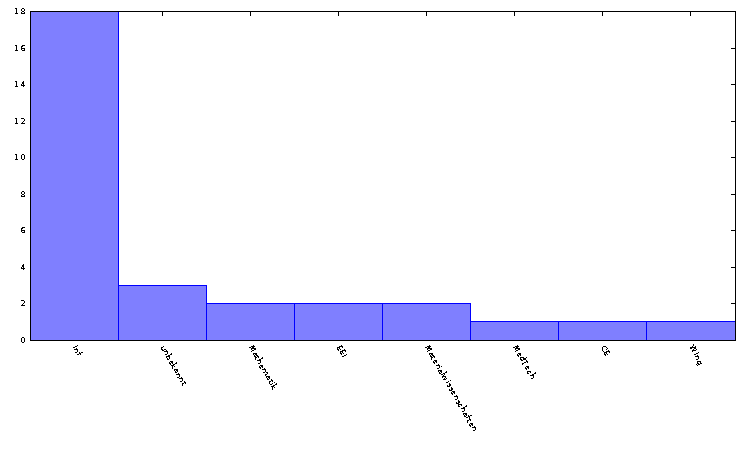
\includegraphics[scale=0.9]{plots/reglm.pdf}
	\end{center}
\end{frame}

\begin{frame}{Details}
	$30$ Befragte, die E-Mail-Kryptographie regelmäßig einsetzen:
  \begin{itemize}
	\item<2-> $29$ finden, dass ihre Software einfach zu bedienen ist
	\item<2-> $1$ Informatiker ($12.$ Semester, E-Mail-Client: Thunderbird, OS: Linux) findet seine Software schwer zu bedienen
	\item<3-> Die Studierenden verschicken im Durchschnitt $8.5$ verschlüsselte Mails im Monat (Standardabw.: $8.3$, Maximum: $30$)
	\item<4-> Die Studierenden haben im Durchschnitt $4.1$ Kontakte, mit denen sie verschlüsselt kommuniziert können
		(Standardabw.: $5.2$, Maximum: $25$)
	\item<5-> $17$ Studierenden nutzen Thunderbird, $8$ OS X Mail, oft in Kombination mit Webclient und Smartphone
  \end{itemize}
\end{frame}


%%%% min 1x eingesetzt

\begin{frame}{Fragebogenverlauf}
	\begin{tikzpicture}[mindmap,scale=0.7]
		\path[concept color=goldenrod,every concept/.append style={scale=0.7}]
		node[concept] {$207$ \\ $100\%$}
			child[concept color=gray,grow=-5] {node[concept] {$65$ \\ $31.40\%$}}
			child[concept color=goldenrod,grow=-170] {node[concept] {$142$ \\ $68,60\%$}
				child[concept color=gray,grow=-30] {node[concept] {}
					child[concept color=gray,grow=-90] {node[concept] {}
						child[concept color=gray,grow=-130] {node[concept] {}}
						child[concept color=gray,grow=-70] {node[concept] {}}
					}
					child[concept color=gray,grow=-10] {node[concept] {}
						child[concept color=gray,grow=0] {node[concept] {}}
						child[concept color=gray,grow=-60] {node[concept] {}
							child[concept color=gray,grow=-130] {node[concept] {}}
							child[concept color=gray,grow=-50] {node[concept] {}}
						}
					}
				}
				child[concept color=goldenrod,grow=-130] {node[concept] {$54$ \\ $26.09\%$}
					child[concept color=gray,grow=-130] {node[concept] {$30$ \\ $14.49\%$}}
					child[concept color=goldenrod,grow=-70] {node[concept] (R) {$24$ \\ $11.59\%$}
						child[concept color=violet!70,grow=-130] {node[concept] {$17$ \\ $8.21\%$}}
						child[concept color=gray,grow=-70] {node[concept] {}
							child[concept color=gray,grow=-130] {node[concept] {}}
							child[concept color=gray,grow=-70] {node[concept] {}}
						}
					}
				}
			};
			\only<1>{
				\draw node[annotation,below,fill=gray!30] (Q) at (-6,2.3) {Haben Sie jemals eine verschlüsselte E-Mail verschickt?};
				\draw [concept connection] (R) edge (Q);
			}
			\only<2>{
				\node[annotation,below,fill=gray!50,scale=1.3] at (4,-6.4) {E-Mail-Kryptographie wurde schon mindestens einmal eingesetzt.};
			}
	\end{tikzpicture}
\end{frame}

\begin{frame}{Details}
	Unter den $17$ Befragten, die schon mindestens einmal eine verschlüsselte E-Mail versendet haben,
	befinden sich $9$ Informatiker.
\end{frame}

\begin{frame}{Details}
	Usability-Probleme, aufgrund deren E-Mailverschlüsselung nicht (regelmäßig) eingesetzt wird:
	\begin{itemize}[<+->]
%    \item Keine meiner Kommunikationspartner hält es für nötig und da zu Verschlüsselung immer zwei gehören, erübrigt sich das ganze Vorhaben.
    %\item Weil ich die Erfahrung gemacht habe, dass der Empfänger, selbst wenn er einen PGP-Key besitzt und veröffentlicht hat,  diese meist nicht entschlüsseln kann, weil er die passende Softwware nicht installiert hat. Meistens ist es wichtiger, dass eine E-Mail ankommt, als dass sie verschlüsselt ist.
    %\item Android-Handy (und GMail Webinterface) unterstützen keine verschlüsselten Mails, insbesondere empfangene, verschlüsselte Mails könnten nicht einmal gelesen werden.
    %\item Im Umfeld außerhalb des Arbeitsplatzes nicht sehr verbreitet.
%Per E-Mail werden daher auch keine wichtigen Informationen versendet.
	  \item Empfänger können trotz des Besitzes eines PGP-Keys nicht entschlüsseln (z.B. wegen fehlender Software)
	  \item Etliche E-Mail-Clients (insb. Webclients) unterstützen keine Verschlüsselung
	  \item Absprache mit Kommunikationspartner und Schlüsseltransfer aufwändig
	  \item Public-Keys selten veröffentlicht, kein praktikables System für Schlüsselweitergabe vorhanden
  \end{itemize}
\end{frame}

\begin{frame}{Details}
	Andere Ursachen, weshalb E-Mail-Verschlüsselung nicht (regelmäßig) eingesetzt wird:
	\begin{itemize}[<+->]
	  \item Kommunikationspartner halten es für unnötig
	  \item Meistens sei es wichtiger, dass eine E-Mail ankommt, als dass sie verschlüsselt ist
	  \item Im privaten Umfeld wenig verbreitet
	  \item In vielen E-Mails werden keine wichtigen (schützenswerten) Informationen versendet
	  \item sensible Daten werden nur persönlich an Vertraute weitergegeben
	\end{itemize}
	
\end{frame}

%%%% noch nie eingesetzt trotz vorhandener kontakte
\begin{frame}{Fragebogenverlauf}
	\begin{tikzpicture}[mindmap,scale=0.7]
		\path[concept color=goldenrod,every concept/.append style={scale=0.7}]
		node[concept] {$207$ \\ $100\%$}
			child[concept color=gray,grow=-5] {node[concept] {$65$ \\ $31.40\%$}}
			child[concept color=goldenrod,grow=-170] {node[concept] {$142$ \\ $68,60\%$}
				child[concept color=gray,grow=-30] {node[concept] {}
					child[concept color=gray,grow=-90] {node[concept] {}
						child[concept color=gray,grow=-130] {node[concept] {}}
						child[concept color=gray,grow=-70] {node[concept] {}}
					}
					child[concept color=gray,grow=-10] {node[concept] {}
						child[concept color=gray,grow=0] {node[concept] {}}
						child[concept color=gray,grow=-60] {node[concept] {}
							child[concept color=gray,grow=-130] {node[concept] {}}
							child[concept color=gray,grow=-50] {node[concept] {}}
						}
					}
				}
				child[concept color=goldenrod,grow=-130] {node[concept] {$54$ \\ $26.09\%$}
					child[concept color=gray,grow=-130] {node[concept] {$30$ \\ $14.49\%$}}
					child[concept color=goldenrod,grow=-70] {node[concept] {$24$ \\ $11.59\%$}
						child[concept color=gray,grow=-130] {node[concept] {$17$ \\ $8.21\%$}}
						child[concept color=goldenrod,grow=-70] {node[concept] (R) {$7$ \\ $3.38\%$}
							child[concept color=red,grow=-130] {node[concept] {$6$ \\ $2.90\%$}}
							child[concept color=gray,grow=-70] {node[concept] {}}
						}
					}
				}
			};
			\only<1>{
				\draw node[annotation,below,fill=gray!30] (Q) at (-6,2.3) {Haben Sie Kontakte, mit denen Sie verschlüsslt kommunizieren können?};
				\draw [concept connection] (R) edge (Q);
			}
			\only<2>{
				\node[annotation,below,fill=gray!50,scale=1.3] at (4,-6.4) {E-Mail-Kryptographie wurde noch nie eingesetzt, obwohl Software und
					Kontakte vorhanden wären, mit denen verschlüsselte Kommunikation möglich wäre.};
			}
	\end{tikzpicture}
\end{frame}

%%%% keine kontakte vorhanden
\begin{frame}{Fragebogenverlauf}
	\begin{tikzpicture}[mindmap,scale=0.7]
		\path[concept color=goldenrod,every concept/.append style={scale=0.7}]
		node[concept] {$207$ \\ $100\%$}
			child[concept color=gray,grow=-5] {node[concept] {$65$ \\ $31.40\%$}}
			child[concept color=goldenrod,grow=-170] {node[concept] {$142$ \\ $68,60\%$}
				child[concept color=gray,grow=-30] {node[concept] {}
					child[concept color=gray,grow=-90] {node[concept] {}
						child[concept color=gray,grow=-130] {node[concept] {}}
						child[concept color=gray,grow=-70] {node[concept] {}}
					}
					child[concept color=gray,grow=-10] {node[concept] {}
						child[concept color=gray,grow=0] {node[concept] {}}
						child[concept color=gray,grow=-60] {node[concept] {}
							child[concept color=gray,grow=-130] {node[concept] {}}
							child[concept color=gray,grow=-50] {node[concept] {}}
						}
					}
				}
				child[concept color=goldenrod,grow=-130] {node[concept] {$54$ \\ $26.09\%$}
					child[concept color=gray,grow=-130] {node[concept] {$30$ \\ $14.49\%$}}
					child[concept color=goldenrod,grow=-70] {node[concept] {$24$ \\ $11.59\%$}
						child[concept color=gray,grow=-130] {node[concept] {$17$ \\ $8.21\%$}}
						child[concept color=goldenrod,grow=-70] {node[concept] {$7$ \\ $3.38\%$}
							child[concept color=gray,grow=-130] {node[concept] {$6$ \\ $2.90\%$}}
							child[concept color=blue!70,grow=-70] {node[concept] {$1$ \\ $0.48\%$}}
						}
					}
				}
			};
			\node[annotation,below,fill=gray!50,scale=1.3] at (4,-6.4) {Keine Kontakte, mit denen verschlüsselte Kommunikation möglich ist, vorhanden.};
	\end{tikzpicture}
\end{frame}

%%%% schonmal installiert, bewusst entfernt
\begin{frame}{Fragebogenverlauf}
	\begin{tikzpicture}[mindmap,scale=0.7]
		\path[concept color=goldenrod,every concept/.append style={scale=0.7}]
		node[concept] {$207$ \\ $100\%$}
			child[concept color=gray,grow=-5] {node[concept] {$65$ \\ $31.40\%$}}
			child[concept color=goldenrod,grow=-170] {node[concept] {$142$ \\ $68,60\%$}
				child[concept color=goldenrod,grow=-30] {node[concept] (R) {$88$ \\ $42.51\%$}
					child[concept color=goldenrod,grow=-90] {node[concept] (R1) {$15$ \\ $7.25\%$}
						child[concept color=red,grow=-130] {node[concept] {$9$ \\ $4.35\%$}}
						child[concept color=gray,grow=-70] {node[concept] {}}
					}
					child[concept color=gray,grow=-10] {node[concept] {}
						child[concept color=gray,grow=0] {node[concept] {}}
						child[concept color=gray,grow=-60] {node[concept] {}
							child[concept color=gray,grow=-130] {node[concept] {}}
							child[concept color=gray,grow=-50] {node[concept] {}}
						}
					}
				}
				child[concept color=gray,grow=-130] {node[concept] {$54$ \\ $26.09\%$}
					child[concept color=gray,grow=-130] {node[concept] {$30$ \\ $14.49\%$}}
					child[concept color=gray,grow=-70] {node[concept] {$24$ \\ $11.59\%$}
						child[concept color=gray,grow=-130] {node[concept] {$17$ \\ $8.21\%$}}
						child[concept color=gray,grow=-70] {node[concept] {$7$ \\ $3.38\%$}
							child[concept color=gray,grow=-130] {node[concept] {$6$ \\ $2.90\%$}}
							child[concept color=gray,grow=-70] {node[concept] {$1$ \\ $0.48\%$}}
						}
					}
				}
			};
			\only<1>{
				\draw node[annotation,below,fill=gray!30] (Q) at (-6,2.3) {War schon einmal Software für E-Mail-Kryptographie installiert?};
				\draw [concept connection] (R) edge (Q);
			}
			\only<2>{
				\draw node[annotation,below,fill=gray!30] (Q) at (-6,2.3) {Haben Sie diese Software bewusst entfernt?};
				\draw [concept connection] (R1) edge (Q1);
			}
			\only<3>{
				\node[annotation,below,fill=gray!50,scale=1.3] at (4,-6.4) {Software für E-Mail-Kryptographie war schonmal installiert, wurde jedoch bewusst wieder entfernt.};
			}
	\end{tikzpicture}
\end{frame}

%%%% schonmal installiert, unbewusst entfernt
\begin{frame}{Fragebogenverlauf}
	\begin{tikzpicture}[mindmap,scale=0.7]
		\path[concept color=goldenrod,every concept/.append style={scale=0.7}]
		node[concept] {$207$ \\ $100\%$}
			child[concept color=gray,grow=-5] {node[concept] {$65$ \\ $31.40\%$}}
			child[concept color=goldenrod,grow=-170] {node[concept] {$142$ \\ $68,60\%$}
				child[concept color=goldenrod,grow=-30] {node[concept] {$88$ \\ $42.51\%$}
					child[concept color=goldenrod,grow=-90] {node[concept] {$15$ \\ $7.25\%$}
						child[concept color=gray,grow=-130] {node[concept] {$9$ \\ $4.35\%$}}
						child[concept color=red,grow=-70] {node[concept] {$6$ \\ $2.90\%$}}
					}
					child[concept color=gray,grow=-10] {node[concept] {}
						child[concept color=gray,grow=0] {node[concept] {}}
						child[concept color=gray,grow=-60] {node[concept] {}
							child[concept color=gray,grow=-130] {node[concept] {}}
							child[concept color=gray,grow=-50] {node[concept] {}}
						}
					}
				}
				child[concept color=gray,grow=-130] {node[concept] {$54$ \\ $26.09\%$}
					child[concept color=gray,grow=-130] {node[concept] {$30$ \\ $14.49\%$}}
					child[concept color=gray,grow=-70] {node[concept] {$24$ \\ $11.59\%$}
						child[concept color=gray,grow=-130] {node[concept] {$17$ \\ $8.21\%$}}
						child[concept color=gray,grow=-70] {node[concept] {$7$ \\ $3.38\%$}
							child[concept color=gray,grow=-130] {node[concept] {$6$ \\ $2.90\%$}}
							child[concept color=gray,grow=-70] {node[concept] {$1$ \\ $0.48\%$}}
						}
					}
				}
			};
			\node[annotation,below,fill=gray!50,scale=1.3] at (4,-6.4) {Software für E-Mail-Kryptographie war schon
			einmal installiert, sie wurde jedoch nicht bewusst entfernt.};
	\end{tikzpicture}
\end{frame}

%%%% schonmal versucht zu installieren // gescheitert
\begin{frame}{Fragebogenverlauf}
	\begin{tikzpicture}[mindmap,scale=0.7]
		\path[concept color=goldenrod,every concept/.append style={scale=0.7}]
		node[concept] {$207$ \\ $100\%$}
			child[concept color=gray,grow=-5] {node[concept] {$65$ \\ $31.40\%$}}
			child[concept color=goldenrod,grow=-170] {node[concept] {$142$ \\ $68,60\%$}
				child[concept color=goldenrod,grow=-30] {node[concept] {$88$ \\ $42.51\%$}
					child[concept color=gray,grow=-90] {node[concept] {$15$ \\ $7.25\%$}
						child[concept color=gray,grow=-130] {node[concept] {$9$ \\ $4.35\%$}}
						child[concept color=gray,grow=-70] {node[concept] {$6$ \\ $2.90\%$}}
					}
					child[concept color=goldenrod,grow=-10] {node[concept] (R) {$73$ \\ $35.27\%$}
						child[concept color=gray,grow=0] {node[concept] { }}
						child[concept color=goldenrod,grow=-60] {node[concept] (R1) {$19$ \\ $9.18\%$}
							child[concept color=red,grow=-130] {node[concept] {$1$ \\ $0.48\%$ }}
							child[concept color=gray,grow=-50] {node[concept] {}}
						}
					}
				}
				child[concept color=gray,grow=-130] {node[concept] {$54$ \\ $26.09\%$}
					child[concept color=gray,grow=-130] {node[concept] {$30$ \\ $14.49\%$}}
					child[concept color=gray,grow=-70] {node[concept] {$24$ \\ $11.59\%$}
						child[concept color=gray,grow=-130] {node[concept] {$17$ \\ $8.21\%$}}
						child[concept color=gray,grow=-70] {node[concept] {$7$ \\ $3.38\%$}
							child[concept color=gray,grow=-130] {node[concept] {$6$ \\ $2.90\%$}}
							child[concept color=gray,grow=-70] {node[concept] {$1$ \\ $0.48\%$}}
						}
					}
				}
			};
			\only<1>{
				\draw node[annotation,below,fill=gray!30] (Q) at (-6,2.3) {Haben Sie schon einmal eine Installation geplant?};
				\draw [concept connection] (R) edge (Q);
			}
			\only<2>{
				\draw node[annotation,below,fill=gray!30] (Q1) at (-6,2.3) {Haben Sie schon einmal eine Installation versucht?};
				\draw [concept connection] (R1) edge (Q1);
			}
			\only<3>{
				\node[annotation,below,fill=gray!50,scale=1.3] at (4,-6.4) {Software für E-Mail-Kryptographie war noch
				nie installiert; es wurde schon einmal versucht, eine solche Software zu installieren (gescheitert).};
			}
	\end{tikzpicture}
\end{frame}

\begin{frame}{Details}
	$1$ Wirtschaftsingenieur ($6.$ Semester, OS: Windows, Client: Thunderbird) hat schon einmal versucht, Software für E-Mail-Kryptographie zu installieren.

	Kommentar: ``Fehler Meldung! Danach hab ichs deinstalliert, weil eh keiner `mitmacht' und sich den Aufwand macht. Wenn keiner Verschlüsselung nutzt lohnt der Aufwand (auch wenns eigentlich keiner ist) nicht es ein zweites Mal zu probieren!''
\end{frame}

%%%% installation geplant aber nie versucht
\begin{frame}{Fragebogenverlauf}
	\begin{tikzpicture}[mindmap,scale=0.7]
		\path[concept color=goldenrod,every concept/.append style={scale=0.7}]
		node[concept] {$207$ \\ $100\%$}
			child[concept color=gray,grow=-5] {node[concept] {$65$ \\ $31.40\%$}}
			child[concept color=goldenrod,grow=-170] {node[concept] {$142$ \\ $68,60\%$}
				child[concept color=goldenrod,grow=-30] {node[concept] {$88$ \\ $42.51\%$}
					child[concept color=gray,grow=-90] {node[concept] {$15$ \\ $7.25\%$}
						child[concept color=gray,grow=-130] {node[concept] {$9$ \\ $4.35\%$}}
						child[concept color=gray,grow=-70] {node[concept] {$6$ \\ $2.90\%$}}
					}
					child[concept color=goldenrod,grow=-10] {node[concept] {$73$ \\ $35.27\%$}
						child[concept color=gray,grow=0] {node[concept] {}}
						child[concept color=goldenrod,grow=-60] {node[concept] {$19$ \\ $9.18\%$}
							child[concept color=gray,grow=-130] {node[concept] {$1$ \\ $0.48\%$}}
							child[concept color=blue!70,grow=-50] {node[concept] {$18$ \\ $8.70\%$}}
						}
					}
				}
				child[concept color=gray,grow=-130] {node[concept] {$54$ \\ $26.09\%$}
					child[concept color=gray,grow=-130] {node[concept] {$30$ \\ $14.49\%$}}
					child[concept color=gray,grow=-70] {node[concept] {$24$ \\ $11.59\%$}
						child[concept color=gray,grow=-130] {node[concept] {$17$ \\ $8.21\%$}}
						child[concept color=gray,grow=-70] {node[concept] {$7$ \\ $3.38\%$}
							child[concept color=gray,grow=-130] {node[concept] {$6$ \\ $2.90\%$}}
							child[concept color=gray,grow=-70] {node[concept] {$1$ \\ $0.48\%$}}
						}
					}
				}
			};
			\node[annotation,below,fill=gray!50,scale=1.3] at (4,-6.4) {Software für E-Mail-Kryptographie war noch nie installiert; Installation war geplant, jedoch nie
			tatsächlich versucht.};
	\end{tikzpicture}
\end{frame}

%%%% installation nie geplant, nie versucht
\begin{frame}{Fragebogenverlauf}
	\begin{tikzpicture}[mindmap,scale=0.7]
		\path[concept color=goldenrod,every concept/.append style={scale=0.7}]
		node[concept] {$207$ \\ $100\%$}
			child[concept color=gray,grow=-5] {node[concept] {$65$ \\ $31.40\%$}}
			child[concept color=goldenrod,grow=-170] {node[concept] {$142$ \\ $68,60\%$}
				child[concept color=goldenrod,grow=-30] {node[concept] {$88$ \\ $42.51\%$}
					child[concept color=gray,grow=-90] {node[concept] {$15$ \\ $7.25\%$}
						child[concept color=gray,grow=-130] {node[concept] {$9$ \\ $4.35\%$}}
						child[concept color=gray,grow=-70] {node[concept] {$6$ \\ $2.90\%$}}
					}
					child[concept color=goldenrod,grow=-10] {node[concept] {$73$ \\ $35.27\%$}
						child[concept color=blue!70,grow=0] {node[concept] {$54$ \\ $26.09\%$}}
						child[concept color=gray,grow=-60] {node[concept] {$19$ \\ $9.18\%$}
							child[concept color=gray,grow=-130] {node[concept] {$1$ \\ $0.48\%$}}
							child[concept color=gray,grow=-50] {node[concept] {$18$ \\ $8.70\%$}}
						}
					}
				}
				child[concept color=gray,grow=-130] {node[concept] {$54$ \\ $26.09\%$}
					child[concept color=gray,grow=-130] {node[concept] {$30$ \\ $14.49\%$}}
					child[concept color=gray,grow=-70] {node[concept] {$24$ \\ $11.59\%$}
						child[concept color=gray,grow=-130] {node[concept] {$17$ \\ $8.21\%$}}
						child[concept color=gray,grow=-70] {node[concept] {$7$ \\ $3.38\%$}
							child[concept color=gray,grow=-130] {node[concept] {$6$ \\ $2.90\%$}}
							child[concept color=gray,grow=-70] {node[concept] {$1$ \\ $0.48\%$}}
						}
					}
				}
			};
			\node[annotation,below,fill=gray!50,scale=1.3] at (4,-6.4) {Software für E-Mail-Kryptographie war noch nie installiert; Installation war nie geplant.};
	\end{tikzpicture}
\end{frame}

\begin{frame}{Details}
	\begin{center}
		Studienfächer
		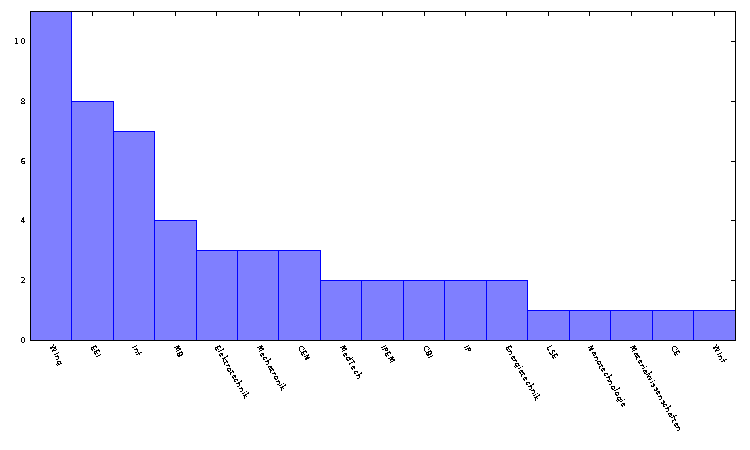
\includegraphics[scale=0.9]{plots/noplan.pdf}
	\end{center}
\end{frame}

\section{Forschungsergebnis}
\begin{frame}{Forschungsergebnis}
\begin{itemize}
	\item Von $207$ befragten setzen $30$ E-Mail-Kryptographie regelmäßig ein
	\item Von den restlichen $177$ werden (konservativ betrachtet) $39$ durch Usability-Probleme
		vom Einsatz von E-Mail-Kryptographie abgehalten; dies entspricht $22.03\%$
	\item $77.97\%$ werden also aus anderen Gründen vom Einsatz von E-Mail-Kryptographie abgehalten
	\item<2> die Hypothese ist somit bestätigt
\end{itemize}
	\only<2>{
		\begin{block}{Hypothese}
			Usability-Probleme von Kryptographie-Software sind
			nicht die primäre Ursache für die geringe Verbreitung von E-Mail-Kryptographie,
			da mehr als 50\% der potenziellen Nutzer durch andere Ursachen davon abgehalten werden, E-Mail-Kryptographie zu nutzen.
		\end{block}
	}
	\only<3>{
		\begin{block}{andere Probleme}
			Unwissen\\
			Desinteresse\\
			mangelnde Motivation\\
			mangelnde Verbreitung von E-Mail-Kryptographie
		\end{block}
	}
\end{frame}

\section{Einschränkungen}
\begin{frame}{Einschränkungen}
	  \begin{itemize}
    \item indirekte Effekte schlechter Usability werden nicht betrachtet
    \item Frage nach dem Begriff ``E-Mail-Kryptographie'' problematisch
    \item nur Studierende aus technischen Fächern befragt
    \item technische Probleme
	\end{itemize}
\end{frame}

\section{Diskussion}
\begin{frame}{Diskussion}
	Was könnte man verbessern? Was könnte man in Folgestudien untersuchen?
	\begin{itemize}[<+->]
		\item Andere Zielgruppen (alle Studierenden an der Universität, Beschäftigte in der Industrie, verschiedene Altersgruppen)
		\item Ergänzung durch detailliertere Fragen
		\item Untersuchung einzelner Phänomene (Einfluss des Rufes von E-Mail-Kryptographie auf die Ergebnisse, o.Ä.)
		\item Wieviele Studierende wissen nicht, was sie studieren? (Studienfach: ``Masters'', ``Lehramt'')\\
			Wieviele Studierende können ihr Studienfach nicht richtig schreiben?
	\end{itemize}
\end{frame}

\begin{frame}{Diskussion}
  \begin{center}
	Fragen?

	Anmerkungen?
    
	Kritik?
    
	Diskussion!
	\end{center}
\end{frame}

\appendix
\section{Appendix}
\subsection*{Detail-Statistiken}
\begin{frame}{Details}
	$65$ Studierende, die den Begriff ``E-Mail-Kryptographie'' nicht kennen:
	\begin{itemize}
		\item Die Studierenden sind im Durchschnitt im $5.1$-ten Semester\\ (Standardabw.: $2.9$, Maximum: $12$)
		\item OS: $53$ nutzen Microsoft Windows, $9$ nutzen Mac OS
		\item E-Mail-Clients: $37$ nutzen Seamonkey, $11$ OS X Mail, $8$ Thunderbird, häufig zusätzliche Nutzung von Webclients, Smartphones
	\end{itemize}
\end{frame}

\begin{frame}{Details}
	$17$ Befragte, die schon mindestens einmal eine verschlüsselte E-Mail versendet haben:
	\begin{itemize}
		\item $9$ Informatiker
		\item $11$ setzen Linux, $3$ Windows, $2$ Mac OS als Betriebssystem ein
		\item $10$ benutzen Thunderbird, $7$ Webclients (oft in Kombination)
		\item Die Befragten sind im Durchschnitt im $6.1$-ten Semester\\(Standardabw.: $2.4$, Maximum: $10$)
	\end{itemize}
\end{frame}


\begin{frame}{Details}
	$6$ Befragte, die trotz vorhandener Kontakte keine verschlüsselten Mails versenden:
	\begin{itemize}
		\item Studienfächer: Informatik ($2$), Nanotechnologie, Maschinenbau, Mechatronik, Materialwissenschaften
		\item Semester: im Durchschnitt $9.0$ (Standardabw.: $3.6$, Maximum: $16$)
		\item Betriebssystem: $4$ Windows, $2$ Linux
		\item E-Mail-Client: Thunderbird, Outlook, Webclient, u.a.
	\end{itemize}
\end{frame}

\begin{frame}{Details}
	$1$ Befragter, der keine Kontakte hat, mit denen er verschlüsselt kommunizieren kann:
	\begin{itemize}
		\item Wirtschaftsingenieur
		\item $6.$ Semester
		\item OS: Linux
		\item E-Mail-Client: Thunderbird
	\end{itemize}
\end{frame}

\begin{frame}{Details}
	$9$ Befragte, die E-Mail-Kryptographie-Software bewusst entfernt haben:
\begin{itemize}
	\item Studienfach: Informatik ($4$), EEI ($2$), WIng ($2$), Maschinenbau
	\item Semester: $7.1$ im Durchschnitt (Standwardabw.: $3.6$, Maximum: $13$)
	\item OS: Windows ($6$), Linux ($2$), Mac OS
	\item E-Mail-Client: Webclient, Thunderbird, u.a.
\end{itemize}
\end{frame}

\begin{frame}{Details}
	$6$ Befragte, die ihre E-Mail-Kryptographie-Software nicht bewusst entfernt haben:
	\begin{itemize}
		\item Studienfach: Informatik ($2$), LSE, Energietechnik, Nanotechnologie
		\item Semester: $5.7$ im Durchschnitt (Standardabw.: $1.8$, Maximum: $8$)
		\item OS: Windows ($4$), Linux
		\item E-Mail-Clients: Webclient, Thunderbird und andere
	\end{itemize}
\end{frame}

\begin{frame}{Details}
	$18$ Befragte hatten zwar schon einmal geplant E-Mail-Kryptographie-Software zu installieren, es jedoch nie tatsächlich versucht:
	\begin{itemize}
		\item Studienfächer: Energietechnik ($3$), Maschinenbau ($3$), Mechatronik ($2$), IIS ($2$), u.a.
		\item Semester: $5.2$ (Standardabw.: $2.6$, Maximum: $12$)
		\item OS: Windows ($16$), Linux ($2$)
		\item E-Mail-Client: Webclient, Thunderbird, u.a.
	\end{itemize}
\end{frame}

\begin{frame}{Details}
	$54$ Befragte, die Software für E-Mail-Kryptographie noch nie installiert hatten und dies auch noch nie geplant haben:
	\begin{itemize}
		\item Semester: $6.6$ (Standardabw.: $3.4$, Maximum: $14$)
		\item OS: Windows ($43$), Mac OS ($8$), Linux ($2$)
		\item E-Mail-Clients: Webclient ($30$), Outlook ($17$), Thunderbird ($11$), u.a. (OS X Mail, Smartphone-Clients, Mutt, \ldots)
	\end{itemize}
\end{frame}


\end{document}
